\begin{frame}{Different Levels of Tokenization}
  \begin{itemize}
    \item[\textcolor{red}{$\blacktriangleright$}] \textbf{Character-level}
    \begin{itemize}
      \item Fine-grained, handles unknowns
      \item Long sequences, slow training
    \end{itemize}
    \vspace{0.35em}
    \item[\textcolor{red}{$\blacktriangleright$}] \textbf{Word-level}
    \begin{itemize}
      \item Intuitive, natural boundaries
      \item Large vocab, OOV (Out-of-Vocab) issues
    \end{itemize}
    \vspace{0.35em}
    \item[\textcolor{red}{$\blacktriangleright$}] \textbf{Subword-level}
    \begin{itemize}
      \item Balance of generalization \& compactness
      \item Requires segmentation algorithm
    \end{itemize}
    \vspace{0.35em}
    \item[\textcolor{red}{$\blacktriangleright$}] \textbf{How subword vocabularies are built}
    \begin{itemize}
      \item BPE, WordPiece, Unigram LM: all learned from the corpus
      \item SentencePiece applies them to raw text, with no pre-tokenizer
    \end{itemize}
  \end{itemize}
\end{frame}


\begin{frame}{Different Levels of Tokenization}
  \centering
  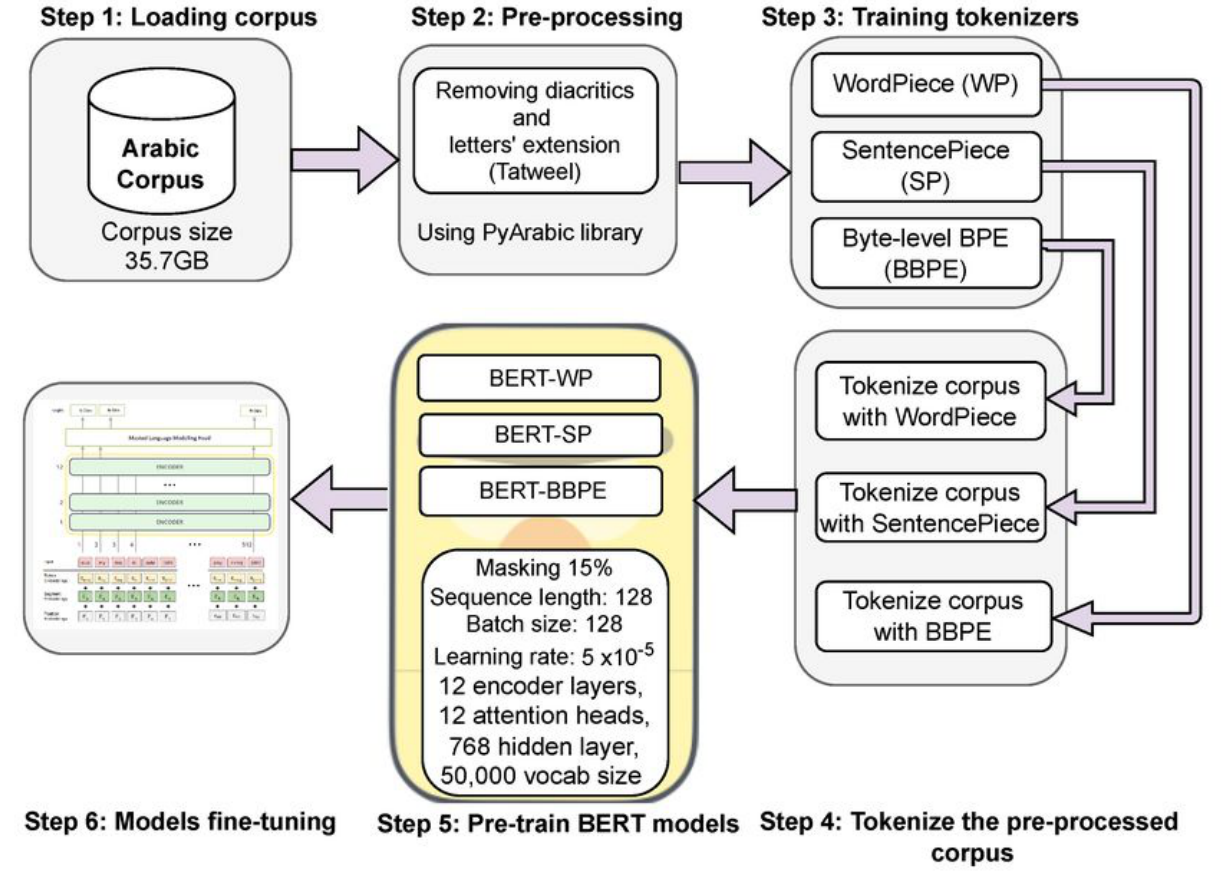
\includegraphics[width=0.60\paperwidth,height=0.60\paperheight,keepaspectratio]{images/large-language-models/llm_arabic_bert_tokenization_pipeline.png}

  {\scriptsize Source: Qarah and Alsanoosy, ``A Comprehensive Analysis of Various Tokenizers for Arabic Large Language Models'', Applied Sciences 14(13), 2024, Fig.~1.}
\end{frame}

\begin{frame}{Different Levels of Tokenization}
  \centering
  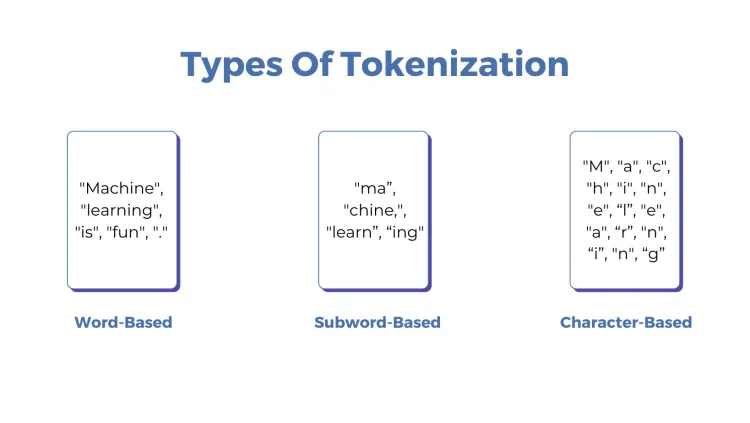
\includegraphics[width=0.60\paperwidth,height=0.60\paperheight,keepaspectratio]{images/large-language-models/llm_word_char_subword_tokenization.png}

  {\scriptsize Source: H. Bui, ``\href{https://eastgate-software.com/insights/what-is-tokenization-in-nlp-everything-you-need-to-understand/}{Tokenization In NLP: Everything We Know So Far}'', Eastgate Software, 2024.}
\end{frame}
